\begin{minipage}{0.49\textwidth}
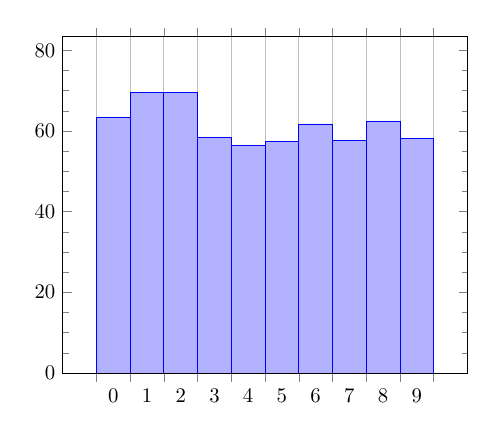
\begin{tikzpicture}[scale=0.75]
  \begin{axis}[ybar interval, ymax=83.3707,ymin=0, minor y tick num = 3]
    \addplot coordinates { (0,63.4862) (1,69.6236) (2,69.6185) (3,58.4626) (4,56.3969) (5,57.3517) (6,61.7428) (7,57.5613) (8,62.4348) (9,58.0804) (10, 37.8958) };
  \end{axis}
\end{tikzpicture}
\caption*{Average weights repartitions on several trees}
\end{minipage}
\begin{minipage}{0.49\textwidth}
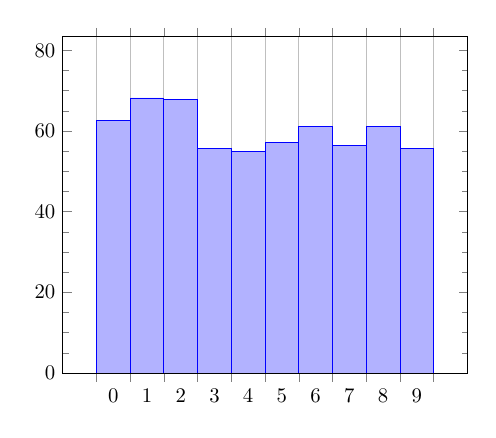
\begin{tikzpicture}[scale=0.75]
  \begin{axis}[ybar interval, ymax=83.3707,ymin=0, minor y tick num = 3]
    \addplot coordinates { (0,62.5682) (1,68.1935) (2,67.9156) (3,55.7816) (4,54.8883) (5,57.0943) (6,61.0943) (7,56.4318) (8,61.1787) (9,55.6352) (10, 37.8958) };
  \end{axis}
\end{tikzpicture}
\caption*{Average weights repartitions on one of the trees}
\end{minipage}
\begin{minipage}{0.49\textwidth}
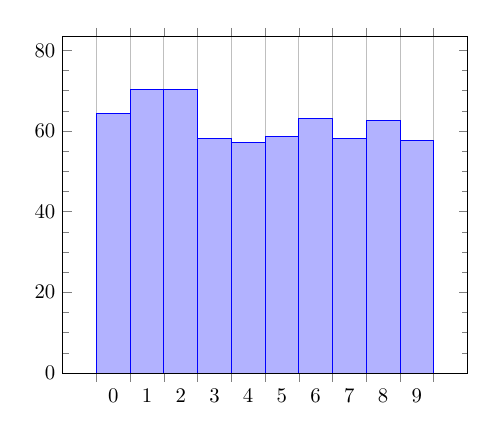
\begin{tikzpicture}[scale=0.75]
  \begin{axis}[ybar interval, ymax=83.3707,ymin=0, minor y tick num = 3]
    \addplot coordinates { (0,64.4367) (1,70.3598) (2,70.2084) (3,58.1737) (4,57.1787) (5,58.6402) (6,63.1811) (7,58.1787) (8,62.7171) (9,57.7593) (10, 37.8958) };
  \end{axis}
\end{tikzpicture}
\caption*{Average weights repartitions on one of the trees}
\end{minipage}
\begin{minipage}{0.49\textwidth}
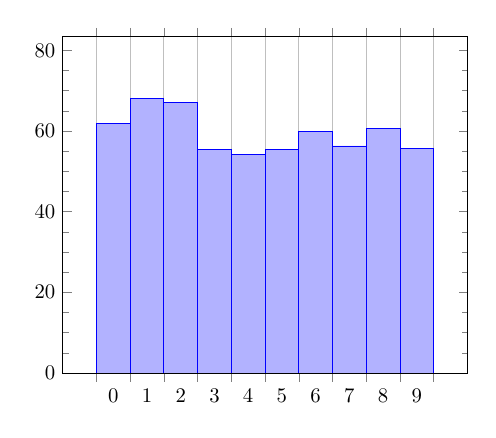
\begin{tikzpicture}[scale=0.75]
  \begin{axis}[ybar interval, ymax=83.3707,ymin=0, minor y tick num = 3]
    \addplot coordinates { (0,61.7568) (1,67.9826) (2,67.0521) (3,55.464) (4,54.2531) (5,55.5087) (6,59.7816) (7,56.2804) (8,60.6551) (9,55.6079) (10, 37.8958) };
  \end{axis}
\end{tikzpicture}
\caption*{Average weights repartitions on one of the trees}
\end{minipage}
